\documentclass{standalone}
\author{Quinten Bruynseraede}
\usepackage{tikz}
\usetikzlibrary{shapes}
\title{Tikz grafen}
\begin{document}\pagestyle{empty}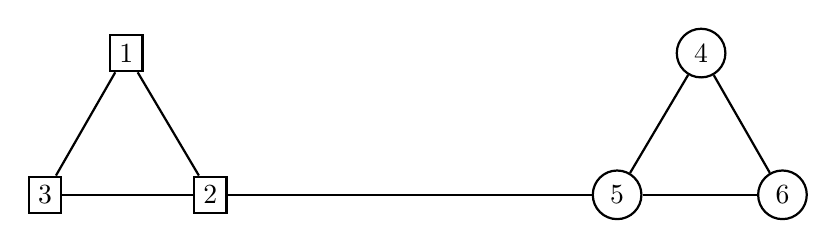
\begin{tikzpicture}\node[shape=rectangle,draw=black,align=center,line width=0.8pt] (0) at (2.066666666666667,13.066666666666666) {1};
\node[shape=rectangle,draw=black,align=center,line width=0.8pt] (1) at (1.0333333333333334,11.266666666666667) {3};
\node[shape=rectangle,draw=black,align=center,line width=0.8pt] (2) at (3.1333333333333333,11.266666666666667) {2};
\node[shape=circle,draw=black,align=center,line width=0.8pt] (3) at (9.366666666666667,13.066666666666666) {4};
\node[shape=circle,draw=black,align=center,line width=0.8pt] (4) at (8.3,11.266666666666667) {5};
\node[shape=circle,draw=black,align=center,line width=0.8pt] (5) at (10.4,11.266666666666667) {6};

\path [-,draw=black,line width=0.8pt] (1) edge node {} (0);
\path [-,draw=black,line width=0.8pt] (0) edge node {} (2);
\path [-,draw=black,line width=0.8pt] (2) edge node {} (1);
\path [-,draw=black,line width=0.8pt] (4) edge node {} (3);
\path [-,draw=black,line width=0.8pt] (3) edge node {} (5);
\path [-,draw=black,line width=0.8pt] (5) edge node {} (4);
\path [-,draw=black,line width=0.8pt] (2) edge node {} (4);
\end{tikzpicture}
\end{document}